\documentclass{beamer}
\usepackage{physics}
\usepackage{amsmath}
\usepackage{tikz}
\usepackage{mathdots}
\usepackage{yhmath}
\usepackage{cancel}
\usepackage{color}
\usepackage{siunitx}
\usepackage{array}
\usepackage{multirow}
\usepackage{amssymb}
\usepackage{textcomp, gensymb}
\usepackage{tabularx}
\usepackage{extarrows}
\usepackage{booktabs}
\usetikzlibrary{fadings}
\usetikzlibrary{patterns}
\usetikzlibrary{shadows.blur}
\usetikzlibrary{shapes}
\usepackage[style=verbose,backend=bibtex]{biblatex}
\addbibresource{arpes.bib}
\addbibresource{green.bib}
\usepackage{listings}
\usepackage{hyperref}

\newcommand{\pair}[1]{\langle #1 \rangle}
\DeclareMathOperator{\ee}{e}
\DeclareMathOperator{\ii}{i}

\newcommand{\concept}[1]{\textbf{#1}}

%region Theme
\usetheme{Madrid}

% Show section in foot
\makeatletter
\setbeamertemplate{footline}
{
  \leavevmode%
  \hbox{%
  \begin{beamercolorbox}[wd=.333333\paperwidth,ht=2.25ex,dp=1ex,center]{author in head/foot}%
    \usebeamerfont{author in head/foot}\insertauthor
  \end{beamercolorbox}%
  \begin{beamercolorbox}[wd=.333333\paperwidth,ht=2.25ex,dp=1ex,center]{title in head/foot}%
    \usebeamerfont{title in head/foot}\insertsection
  \end{beamercolorbox}%
  \begin{beamercolorbox}[wd=.333333\paperwidth,ht=2.25ex,dp=1ex,right]{date in head/foot}%
    \usebeamerfont{date in head/foot}\insertshortdate{}\hspace*{2em}
    \insertframenumber{} / \inserttotalframenumber\hspace*{2ex} 
  \end{beamercolorbox}}%
  \vskip0pt%
}
\makeatother

%endregion

%Information to be included in the title page:
\title{Bosonic modes in Fermi liquid}
\author{Jinyuan Wu}

\begin{document}

\frame{\titlepage}

\section{Introduction}

\begin{frame}
\frametitle{Background}

In a Fermi liquid we have \dots
\begin{itemize}
    \item Quasiparticles (electron/hole) with $\Sigma$-correction
    \item Any anything else?
\end{itemize}    

\begin{center}
    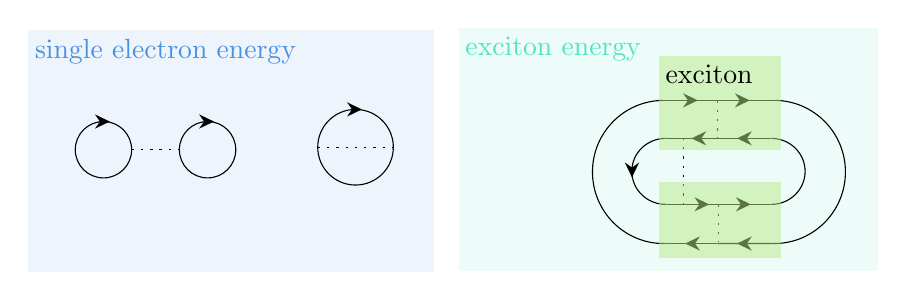
\begin{tikzpicture}[x=0.75pt,y=0.75pt,yscale=-1,xscale=1]
    %uncomment if require: \path (0,300); %set diagram left start at 0, and has height of 300
    
    %Shape: Rectangle [id:dp5146811729500922] 
    \draw  [draw opacity=0][fill={rgb, 255:red, 80; green, 227; blue, 194 }  ,fill opacity=0.1 ] (295.08,59.22) -- (497.25,59.22) -- (497.25,176.41) -- (295.08,176.41) -- cycle ;
    %Straight Lines [id:da6398455748193317] 
    \draw    (407.22,93.98) -- (407.28,93.98) ;
    \draw [shift={(410.28,93.98)}, rotate = 180] [fill={rgb, 255:red, 0; green, 0; blue, 0 }  ][line width=0.08]  [draw opacity=0] (7.14,-3.43) -- (0,0) -- (7.14,3.43) -- (4.74,0) -- cycle    ;
    %Straight Lines [id:da34436720244170616] 
    \draw    (393.72,93.98) -- (419.72,93.98) ;
    %Straight Lines [id:da5378870304376917] 
    \draw  [dash pattern={on 0.84pt off 2.51pt}]  (419.72,93.98) -- (419.72,112.28) ;
    %Straight Lines [id:da6880866744261185] 
    \draw    (432.22,93.98) -- (432.28,93.98) ;
    \draw [shift={(435.28,93.98)}, rotate = 180] [fill={rgb, 255:red, 0; green, 0; blue, 0 }  ][line width=0.08]  [draw opacity=0] (7.14,-3.43) -- (0,0) -- (7.14,3.43) -- (4.74,0) -- cycle    ;
    %Straight Lines [id:da08717980225255384] 
    \draw    (419.72,93.98) -- (447.27,93.98) ;
    %Straight Lines [id:da850721537949833] 
    \draw    (432.22,112.28) -- (432.17,112.28) ;
    \draw [shift={(429.17,112.28)}, rotate = 360] [fill={rgb, 255:red, 0; green, 0; blue, 0 }  ][line width=0.08]  [draw opacity=0] (7.14,-3.43) -- (0,0) -- (7.14,3.43) -- (4.74,0) -- cycle    ;
    %Straight Lines [id:da8852766962819558] 
    \draw    (445.72,112.28) -- (419.72,112.28) ;
    %Straight Lines [id:da2830293714598453] 
    \draw    (410.28,112.28) -- (410.22,112.28) ;
    \draw [shift={(407.22,112.28)}, rotate = 360] [fill={rgb, 255:red, 0; green, 0; blue, 0 }  ][line width=0.08]  [draw opacity=0] (7.14,-3.43) -- (0,0) -- (7.14,3.43) -- (4.74,0) -- cycle    ;
    %Straight Lines [id:da4409957948094987] 
    \draw    (419.72,112.28) -- (394.72,112.28) ;
    %Straight Lines [id:da166206845135215] 
    \draw    (378.56,127.98) -- (378.56,128.08) ;
    \draw [shift={(378.56,131.08)}, rotate = 270] [fill={rgb, 255:red, 0; green, 0; blue, 0 }  ][line width=0.08]  [draw opacity=0] (7.14,-3.43) -- (0,0) -- (7.14,3.43) -- (4.74,0) -- cycle    ;
    %Straight Lines [id:da8858104612113908] 
    \draw    (395.22,144.07) -- (420.22,144.07) ;
    %Straight Lines [id:da7115305058801602] 
    \draw  [dash pattern={on 0.84pt off 2.51pt}]  (420.22,144.07) -- (420.22,162.38) ;
    %Straight Lines [id:da4365031995623925] 
    \draw    (432.72,144.07) -- (432.77,144.07) ;
    \draw [shift={(435.77,144.07)}, rotate = 180] [fill={rgb, 255:red, 0; green, 0; blue, 0 }  ][line width=0.08]  [draw opacity=0] (7.14,-3.43) -- (0,0) -- (7.14,3.43) -- (4.74,0) -- cycle    ;
    %Straight Lines [id:da5381005184479546] 
    \draw    (420.22,144.07) -- (445.22,144.07) ;
    %Straight Lines [id:da5357673686633508] 
    \draw    (432.22,162.95) -- (432.17,162.95) ;
    \draw [shift={(429.17,162.95)}, rotate = 360] [fill={rgb, 255:red, 0; green, 0; blue, 0 }  ][line width=0.08]  [draw opacity=0] (7.14,-3.43) -- (0,0) -- (7.14,3.43) -- (4.74,0) -- cycle    ;
    %Straight Lines [id:da7809394137927026] 
    \draw    (446.19,162.94) -- (419.72,162.95) ;
    %Straight Lines [id:da0014751437976323611] 
    \draw    (407.22,162.95) -- (407.17,162.95) ;
    \draw [shift={(404.17,162.95)}, rotate = 360] [fill={rgb, 255:red, 0; green, 0; blue, 0 }  ][line width=0.08]  [draw opacity=0] (7.14,-3.43) -- (0,0) -- (7.14,3.43) -- (4.74,0) -- cycle    ;
    %Straight Lines [id:da4139281131726549] 
    \draw    (419.72,162.95) -- (394.72,162.95) ;
    %Shape: Arc [id:dp842942564916912] 
    \draw  [draw opacity=0] (395.22,144.07) .. controls (395.08,144.07) and (394.95,144.08) .. (394.81,144.08) .. controls (385.78,144.08) and (378.47,136.96) .. (378.47,128.18) .. controls (378.47,119.43) and (385.74,112.33) .. (394.72,112.28) -- (394.81,128.18) -- cycle ; \draw   (395.22,144.07) .. controls (395.08,144.07) and (394.95,144.08) .. (394.81,144.08) .. controls (385.78,144.08) and (378.47,136.96) .. (378.47,128.18) .. controls (378.47,119.43) and (385.74,112.33) .. (394.72,112.28) ;  
    %Straight Lines [id:da7052800705155782] 
    \draw  [dash pattern={on 0.84pt off 2.51pt}]  (403.39,111.98) -- (403.39,143.41) ;
    %Straight Lines [id:da7494886948705168] 
    \draw    (412.72,144.07) -- (412.77,144.07) ;
    \draw [shift={(415.77,144.07)}, rotate = 180] [fill={rgb, 255:red, 0; green, 0; blue, 0 }  ][line width=0.08]  [draw opacity=0] (7.14,-3.43) -- (0,0) -- (7.14,3.43) -- (4.74,0) -- cycle    ;
    %Shape: Arc [id:dp6452390768047809] 
    \draw  [draw opacity=0] (445.22,144.07) .. controls (445.36,144.07) and (445.49,144.08) .. (445.63,144.08) .. controls (454.65,144.08) and (461.97,136.96) .. (461.97,128.18) .. controls (461.97,119.43) and (454.7,112.33) .. (445.72,112.28) -- (445.63,128.18) -- cycle ; \draw   (445.22,144.07) .. controls (445.36,144.07) and (445.49,144.08) .. (445.63,144.08) .. controls (454.65,144.08) and (461.97,136.96) .. (461.97,128.18) .. controls (461.97,119.43) and (454.7,112.33) .. (445.72,112.28) ;  
    %Shape: Arc [id:dp43945222094751113] 
    \draw  [draw opacity=0] (446.19,162.94) .. controls (446.49,162.95) and (446.78,162.95) .. (447.08,162.95) .. controls (466.03,162.95) and (481.39,147.51) .. (481.39,128.46) .. controls (481.39,109.48) and (466.13,94.08) .. (447.27,93.98) -- (447.08,128.46) -- cycle ; \draw   (446.19,162.94) .. controls (446.49,162.95) and (446.78,162.95) .. (447.08,162.95) .. controls (466.03,162.95) and (481.39,147.51) .. (481.39,128.46) .. controls (481.39,109.48) and (466.13,94.08) .. (447.27,93.98) ;  
    %Shape: Arc [id:dp9293716217993426] 
    \draw  [draw opacity=0] (394.72,162.95) .. controls (394.43,162.96) and (394.13,162.96) .. (393.83,162.96) .. controls (374.88,162.96) and (359.52,147.52) .. (359.52,128.47) .. controls (359.52,109.49) and (374.78,94.09) .. (393.64,93.99) -- (393.83,128.47) -- cycle ; \draw   (394.72,162.95) .. controls (394.43,162.96) and (394.13,162.96) .. (393.83,162.96) .. controls (374.88,162.96) and (359.52,147.52) .. (359.52,128.47) .. controls (359.52,109.49) and (374.78,94.09) .. (393.64,93.99) ;  
    %Shape: Rectangle [id:dp7966285154601207] 
    \draw  [draw opacity=0][fill={rgb, 255:red, 184; green, 233; blue, 134 }  ,fill opacity=0.5 ] (391.5,72.52) -- (450.5,72.52) -- (450.5,117.67) -- (391.5,117.67) -- cycle ;
    %Shape: Rectangle [id:dp15539312444775466] 
    \draw  [draw opacity=0][fill={rgb, 255:red, 184; green, 233; blue, 134 }  ,fill opacity=0.5 ] (391.5,133.52) -- (450.5,133.52) -- (450.5,169.81) -- (391.5,169.81) -- cycle ;
    
    %Shape: Rectangle [id:dp27994217946502586] 
    \draw  [draw opacity=0][fill={rgb, 255:red, 74; green, 144; blue, 226 }  ,fill opacity=0.1 ] (87.67,60.09) -- (283.39,60.09) -- (283.39,176.85) -- (87.67,176.85) -- cycle ;
    %Shape: Circle [id:dp462236419122503] 
    \draw   (110.33,117.75) .. controls (110.33,110.25) and (116.41,104.17) .. (123.92,104.17) .. controls (131.42,104.17) and (137.5,110.25) .. (137.5,117.75) .. controls (137.5,125.25) and (131.42,131.33) .. (123.92,131.33) .. controls (116.41,131.33) and (110.33,125.25) .. (110.33,117.75) -- cycle ;
    %Straight Lines [id:da670513630425587] 
    \draw  [dash pattern={on 0.84pt off 2.51pt}]  (137.5,117.75) -- (160.5,117.75) ;
    %Shape: Circle [id:dp7720535201865808] 
    \draw   (160.5,117.75) .. controls (160.5,110.25) and (166.58,104.17) .. (174.08,104.17) .. controls (181.59,104.17) and (187.67,110.25) .. (187.67,117.75) .. controls (187.67,125.25) and (181.59,131.33) .. (174.08,131.33) .. controls (166.58,131.33) and (160.5,125.25) .. (160.5,117.75) -- cycle ;
    %Straight Lines [id:da8207419794627446] 
    \draw    (174.08,104.17) -- (174.14,104.17) ;
    \draw [shift={(177.14,104.17)}, rotate = 180] [fill={rgb, 255:red, 0; green, 0; blue, 0 }  ][line width=0.08]  [draw opacity=0] (7.14,-3.43) -- (0,0) -- (7.14,3.43) -- (4.74,0) -- cycle    ;
    %Straight Lines [id:da15224804787584634] 
    \draw    (123.92,104.17) -- (123.97,104.17) ;
    \draw [shift={(126.97,104.17)}, rotate = 180] [fill={rgb, 255:red, 0; green, 0; blue, 0 }  ][line width=0.08]  [draw opacity=0] (7.14,-3.43) -- (0,0) -- (7.14,3.43) -- (4.74,0) -- cycle    ;
    
    %Shape: Circle [id:dp2405384911845121] 
    \draw   (227.15,116.55) .. controls (227.15,106.49) and (235.3,98.33) .. (245.36,98.33) .. controls (255.43,98.33) and (263.58,106.49) .. (263.58,116.55) .. controls (263.58,126.61) and (255.43,134.77) .. (245.36,134.77) .. controls (235.3,134.77) and (227.15,126.61) .. (227.15,116.55) -- cycle ;
    %Straight Lines [id:da004084517255771747] 
    \draw  [dash pattern={on 0.84pt off 2.51pt}]  (227.15,116.55) -- (236.71,116.55) -- (263.58,116.55) ;
    %Straight Lines [id:da2452546368901709] 
    \draw    (245.36,98.33) -- (245.42,98.33) ;
    \draw [shift={(248.42,98.33)}, rotate = 180] [fill={rgb, 255:red, 0; green, 0; blue, 0 }  ][line width=0.08]  [draw opacity=0] (7.14,-3.43) -- (0,0) -- (7.14,3.43) -- (4.74,0) -- cycle    ;
    
    
    % Text Node
    \draw (89.67,63.09) node [anchor=north west][inner sep=0.75pt]  [color={rgb, 255:red, 74; green, 144; blue, 226 }  ,opacity=1 ] [align=left] {single electron energy};
    % Text Node
    \draw (393.5,75.52) node [anchor=north west][inner sep=0.75pt]   [align=left] {exciton};
    % Text Node
    \draw (297.08,62.22) node [anchor=north west][inner sep=0.75pt]  [color={rgb, 255:red, 80; green, 227; blue, 194 }  ,opacity=1 ] [align=left] {exciton energy};
    
    
    \end{tikzpicture}
    
\end{center}

\dots and more

\end{frame}

\begin{frame}
\frametitle{Question}

\onslide<1->{
    \textbf{What to do}

    Finding modes other than the corrected single electron/hole   
    
    \vspace{0.6cm}

    \textbf{Why it's important} 
    
    Usually not for $C_V$ but for optical response: $\epsilon$, $\chi^{(3)}$, etc.
}

\onslide<2->{
    \vspace{0.6cm}

    \textbf{Today's topic}

    Electron-hole bosonic modes in Fermi liquid 
    (with \emph{some} scattering picked up back, i.e. 
    beyond $\var{E} \sim \varepsilon \var{n} + f \var{n} \var{n}$), i.e.
    \begin{equation}
        \protect\ket*{\text{single excitation}} = \sum _{\boldsymbol{k}_{1} ,\boldsymbol{k}_{2}} c_{\boldsymbol{k}_{1}\boldsymbol{k}_{2}}\ket{\tikzset{every picture/.style={line width=0.75pt}} %set default line width to 0.75pt        
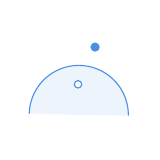
\begin{tikzpicture}[x=0.75pt,y=0.75pt,yscale=-0.5,xscale=0.5, baseline=(XXXX.south) ]
\path (0,100);\path (100,0);\draw    ($(current bounding box.center)+(0,0.3em)$) node [anchor=south] (XXXX) {};
%Shape: Arc [id:dp8520886122690758] 
\draw  [draw opacity=0][fill={rgb, 255:red, 74; green, 144; blue, 226 }  ,fill opacity=0.1 ] (1.48,82.71) .. controls (1.97,66.38) and (10.83,50.73) .. (26.17,42.28) .. controls (49.27,29.54) and (78.33,37.94) .. (91.06,61.04) .. controls (95.22,68.59) and (97.13,76.77) .. (97,84.81) -- (49.23,84.11) -- cycle ; \draw  [color={rgb, 255:red, 74; green, 144; blue, 226 }  ,draw opacity=1 ] (1.48,82.71) .. controls (1.97,66.38) and (10.83,50.73) .. (26.17,42.28) .. controls (49.27,29.54) and (78.33,37.94) .. (91.06,61.04) .. controls (95.22,68.59) and (97.13,76.77) .. (97,84.81) ;  
%Straight Lines [id:da9414882934326914] 
\draw [color={rgb, 255:red, 74; green, 144; blue, 226 }  ,draw opacity=1 ]   (64.93,18.71) ;
\draw [shift={(64.93,18.71)}, rotate = 0] [color={rgb, 255:red, 74; green, 144; blue, 226 }  ,draw opacity=1 ][fill={rgb, 255:red, 74; green, 144; blue, 226 }  ,fill opacity=1 ][line width=0.75]      (0, 0) circle [x radius= 3.35, y radius= 3.35]   ;
%Shape: Circle [id:dp32914036484275444] 
\draw  [color={rgb, 255:red, 74; green, 144; blue, 226 }  ,draw opacity=1 ][fill={rgb, 255:red, 255; green, 255; blue, 255 }  ,fill opacity=1 ] (44.93,54.6) .. controls (44.93,52.62) and (46.53,51.01) .. (48.51,51.01) .. controls (50.49,51.01) and (52.1,52.62) .. (52.1,54.6) .. controls (52.1,56.58) and (50.49,58.18) .. (48.51,58.18) .. controls (46.53,58.18) and (44.93,56.58) .. (44.93,54.6) -- cycle ;
\end{tikzpicture}
}
    \end{equation}

    No trion, higher order correlation, or even more exotic spinons, etc. beyond Fermi liquid
}

\end{frame}

\begin{frame}
\frametitle{Methodology}

\onslide<1->{
\textbf{Series calculation} 

Bethe–Salpeter equation (BSE) is for quantitative calculations. 

\begin{equation}
    \protect\tikzset{every picture/.style={line width=0.75pt}} %set default line width to 0.75pt        
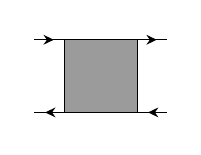
\begin{tikzpicture}[x=0.75pt,y=0.75pt,yscale=-0.7,xscale=0.7, baseline=(XXXX.south) ]
\path (0,68);\path (100,0);\draw    ($(current bounding box.center)+(0,0.3em)$) node [anchor=south] (XXXX) {};
%Straight Lines [id:da22806809134155182] 
\draw    (4.5,8.33) -- (25.33,8.33) ;
%Shape: Square [id:dp6031954177008783] 
\draw  [fill={rgb, 255:red, 155; green, 155; blue, 155 }  ,fill opacity=1 ] (25.33,8.33) -- (75.33,8.33) -- (75.33,58.33) -- (25.33,58.33) -- cycle ;
%Straight Lines [id:da15762936919893056] 
\draw    (14.92,8.33) -- (14.97,8.33) ;
\draw [shift={(17.97,8.33)}, rotate = 180] [fill={rgb, 255:red, 0; green, 0; blue, 0 }  ][line width=0.08]  [draw opacity=0] (7.14,-3.43) -- (0,0) -- (7.14,3.43) -- (4.74,0) -- cycle    ;
%Straight Lines [id:da5710396640221285] 
\draw    (75.33,8.33) -- (96.17,8.33) ;
%Straight Lines [id:da22008735912775146] 
\draw    (85.75,8.33) -- (85.81,8.33) ;
\draw [shift={(88.81,8.33)}, rotate = 180] [fill={rgb, 255:red, 0; green, 0; blue, 0 }  ][line width=0.08]  [draw opacity=0] (7.14,-3.43) -- (0,0) -- (7.14,3.43) -- (4.74,0) -- cycle    ;
%Straight Lines [id:da10139312138178957] 
\draw    (4.5,58.33) -- (25.33,58.33) ;
%Straight Lines [id:da40962399415083883] 
\draw    (14.92,58.33) ;
\draw [shift={(12.04,58.33)}, rotate = 360] [fill={rgb, 255:red, 0; green, 0; blue, 0 }  ][line width=0.08]  [draw opacity=0] (7.14,-3.43) -- (0,0) -- (7.14,3.43) -- (4.74,0) -- cycle    ;
%Straight Lines [id:da7345734656357314] 
\draw    (85.75,58.33) ;
\draw [shift={(82.87,58.33)}, rotate = 360] [fill={rgb, 255:red, 0; green, 0; blue, 0 }  ][line width=0.08]  [draw opacity=0] (7.14,-3.43) -- (0,0) -- (7.14,3.43) -- (4.74,0) -- cycle    ;
%Straight Lines [id:da9940525711272465] 
\draw    (75.33,58.33) -- (96.17,58.33) ;
\end{tikzpicture}
=\tikzset{every picture/.style={line width=0.75pt}} %set default line width to 0.75pt        
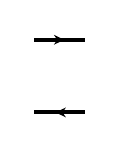
\begin{tikzpicture}[x=0.75pt,y=0.75pt,yscale=-0.7,xscale=0.7, baseline=(XXXX.south) ]
\path (0,68);\path (48.833335876464844,0);\draw    ($(current bounding box.center)+(0,0.3em)$) node [anchor=south] (XXXX) {};
%Straight Lines [id:da5265311146690066] 
\draw [line width=1.5]    (4.5,58.33) -- (39.7,58.33) ;
%Straight Lines [id:da39247742063916924] 
\draw [line width=1.5]    (4.5,8.33) -- (39.7,8.33) ;
%Straight Lines [id:da8442625080101569] 
\draw    (22.1,8.33) -- (22.15,8.33) ;
\draw [shift={(25.15,8.33)}, rotate = 180] [fill={rgb, 255:red, 0; green, 0; blue, 0 }  ][line width=0.08]  [draw opacity=0] (7.14,-3.43) -- (0,0) -- (7.14,3.43) -- (4.74,0) -- cycle    ;
%Straight Lines [id:da3954126655033694] 
\draw    (22.1,58.33) ;
\draw [shift={(19.22,58.33)}, rotate = 360] [fill={rgb, 255:red, 0; green, 0; blue, 0 }  ][line width=0.08]  [draw opacity=0] (7.14,-3.43) -- (0,0) -- (7.14,3.43) -- (4.74,0) -- cycle    ;
\end{tikzpicture}
+\tikzset{every picture/.style={line width=0.75pt}} %set default line width to 0.75pt        
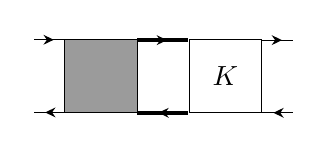
\begin{tikzpicture}[x=0.75pt,y=0.75pt,yscale=-0.7,xscale=0.7, baseline=(XXXX.south) ]
\path (0,68);\path (190.6666717529297,0);\draw    ($(current bounding box.center)+(0,0.3em)$) node [anchor=south] (XXXX) {};
%Straight Lines [id:da7911155113251196] 
\draw    (4.5,8.33) -- (25.33,8.33) ;
%Shape: Square [id:dp19428573744734168] 
\draw  [fill={rgb, 255:red, 155; green, 155; blue, 155 }  ,fill opacity=1 ] (25.33,8.33) -- (75.33,8.33) -- (75.33,58.33) -- (25.33,58.33) -- cycle ;
%Straight Lines [id:da7010679581498145] 
\draw    (14.92,8.33) -- (14.97,8.33) ;
\draw [shift={(17.97,8.33)}, rotate = 180] [fill={rgb, 255:red, 0; green, 0; blue, 0 }  ][line width=0.08]  [draw opacity=0] (7.14,-3.43) -- (0,0) -- (7.14,3.43) -- (4.74,0) -- cycle    ;
%Straight Lines [id:da8907255106568688] 
\draw    (161.58,8.58) -- (182.42,8.58) ;
%Straight Lines [id:da25112705787998446] 
\draw    (172,8.58) -- (172.06,8.58) ;
\draw [shift={(175.06,8.58)}, rotate = 180] [fill={rgb, 255:red, 0; green, 0; blue, 0 }  ][line width=0.08]  [draw opacity=0] (7.14,-3.43) -- (0,0) -- (7.14,3.43) -- (4.74,0) -- cycle    ;
%Straight Lines [id:da15475660740271446] 
\draw    (172,58.58) ;
\draw [shift={(169.12,58.58)}, rotate = 360] [fill={rgb, 255:red, 0; green, 0; blue, 0 }  ][line width=0.08]  [draw opacity=0] (7.14,-3.43) -- (0,0) -- (7.14,3.43) -- (4.74,0) -- cycle    ;
%Straight Lines [id:da5842351849562553] 
\draw    (161.58,58.58) -- (182.42,58.58) ;
%Straight Lines [id:da7087700682172653] 
\draw    (4.5,58.33) -- (25.33,58.33) ;
%Straight Lines [id:da49703420824140654] 
\draw    (14.92,58.33) ;
\draw [shift={(12.04,58.33)}, rotate = 360] [fill={rgb, 255:red, 0; green, 0; blue, 0 }  ][line width=0.08]  [draw opacity=0] (7.14,-3.43) -- (0,0) -- (7.14,3.43) -- (4.74,0) -- cycle    ;
%Straight Lines [id:da5594862502970488] 
\draw [line width=1.5]    (75.25,58.58) -- (110.45,58.58) ;
%Straight Lines [id:da7706538069595303] 
\draw [line width=1.5]    (75.25,8.58) -- (110.45,8.58) ;
%Straight Lines [id:da49897124888842126] 
\draw    (92.85,8.58) -- (92.9,8.58) ;
\draw [shift={(95.9,8.58)}, rotate = 180] [fill={rgb, 255:red, 0; green, 0; blue, 0 }  ][line width=0.08]  [draw opacity=0] (7.14,-3.43) -- (0,0) -- (7.14,3.43) -- (4.74,0) -- cycle    ;
%Straight Lines [id:da896337553631787] 
\draw    (92.85,58.58) ;
\draw [shift={(89.97,58.58)}, rotate = 360] [fill={rgb, 255:red, 0; green, 0; blue, 0 }  ][line width=0.08]  [draw opacity=0] (7.14,-3.43) -- (0,0) -- (7.14,3.43) -- (4.74,0) -- cycle    ;
%Shape: Square [id:dp2523741527250978] 
\draw  [fill={rgb, 255:red, 255; green, 255; blue, 255 }  ,fill opacity=1 ] (111.08,8.33) -- (161.08,8.33) -- (161.08,58.33) -- (111.08,58.33) -- cycle ;
% Text Node
\draw (136.08,33.33) node    {$K$};
\end{tikzpicture}
\end{equation}

\emph{Problem}: no picture about ``how the electron moves''
}

\onslide<2->{
    \vspace{0.5cm}

    \textbf{Linking BSE with single-electron kinetic theory}
    
    Linear response of single-electron under external field = BSE
    
    \begin{equation}
        \protect\Sigma =\tikzset{every picture/.style={line width=0.75pt}} %set default line width to 0.75pt        
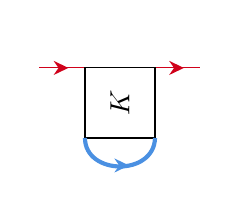
\begin{tikzpicture}[x=0.75pt,y=0.75pt,yscale=-1,xscale=1, baseline=(XXXX.south) ]
\path (0,77);\path (89.33333587646484,0);\draw    ($(current bounding box.center)+(0,0.3em)$) node [anchor=south] (XXXX) {};
%Straight Lines [id:da8382131249777933] 
\draw [color={rgb, 255:red, 208; green, 2; blue, 27 }  ,draw opacity=1 ]   (5.5,19.39) -- (27.61,19.39) ;
%Straight Lines [id:da7240261607790925] 
\draw [color={rgb, 255:red, 208; green, 2; blue, 27 }  ,draw opacity=1 ]   (61.36,19.39) -- (83.06,19.39) ;
%Straight Lines [id:da1930777146623066] 
\draw [color={rgb, 255:red, 208; green, 2; blue, 27 }  ,draw opacity=1 ]   (16.56,19.39) -- (16.61,19.39) ;
\draw [shift={(19.61,19.39)}, rotate = 180] [fill={rgb, 255:red, 208; green, 2; blue, 27 }  ,fill opacity=1 ][line width=0.08]  [draw opacity=0] (7.14,-3.43) -- (0,0) -- (7.14,3.43) -- (4.74,0) -- cycle    ;
%Straight Lines [id:da07919795645711414] 
\draw [color={rgb, 255:red, 208; green, 2; blue, 27 }  ,draw opacity=1 ]   (72.21,19.39) -- (72.27,19.39) ;
\draw [shift={(75.27,19.39)}, rotate = 180] [fill={rgb, 255:red, 208; green, 2; blue, 27 }  ,fill opacity=1 ][line width=0.08]  [draw opacity=0] (7.14,-3.43) -- (0,0) -- (7.14,3.43) -- (4.74,0) -- cycle    ;
%Shape: Square [id:dp5873383974217354] 
\draw   (27.61,19.39) -- (61.36,19.39) -- (61.36,53.14) -- (27.61,53.14) -- cycle ;
%Curve Lines [id:da4568403322032253] 
\draw [color={rgb, 255:red, 74; green, 144; blue, 226 }  ,draw opacity=1 ][line width=1.5]    (27.61,53.14) .. controls (27.61,71.19) and (60.86,71.69) .. (61.36,53.14) ;
%Straight Lines [id:da7186505275056507] 
\draw [color={rgb, 255:red, 74; green, 144; blue, 226 }  ,draw opacity=1 ]   (45.81,66.39) -- (45.86,66.39) ;
\draw [shift={(48.86,66.39)}, rotate = 180] [fill={rgb, 255:red, 74; green, 144; blue, 226 }  ,fill opacity=1 ][line width=0.08]  [draw opacity=0] (7.14,-3.43) -- (0,0) -- (7.14,3.43) -- (4.74,0) -- cycle    ;
% Text Node
\draw (44.49,36.26) node  [rotate=-270]  {$K$};
\end{tikzpicture}
\stackrel{\text{driving}}{\longrightarrow }\tikzset{every picture/.style={line width=0.75pt}} %set default line width to 0.75pt        
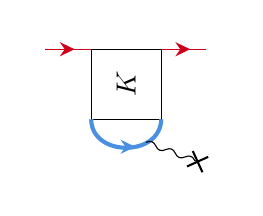
\begin{tikzpicture}[x=0.75pt,y=0.75pt,yscale=-1,xscale=1, baseline=(XXXX.south) ]
\path (0,77);\path (100,0);\draw    ($(current bounding box.center)+(0,0.3em)$) node [anchor=south] (XXXX) {};
%Straight Lines [id:da7828028568002114] 
\draw [color={rgb, 255:red, 208; green, 2; blue, 27 }  ,draw opacity=1 ]   (8.5,10.39) -- (30.61,10.39) ;
%Straight Lines [id:da5090451707270729] 
\draw [color={rgb, 255:red, 208; green, 2; blue, 27 }  ,draw opacity=1 ]   (64.36,10.39) -- (86.06,10.39) ;
%Straight Lines [id:da54602000208046] 
\draw [color={rgb, 255:red, 208; green, 2; blue, 27 }  ,draw opacity=1 ]   (19.56,10.39) -- (19.61,10.39) ;
\draw [shift={(22.61,10.39)}, rotate = 180] [fill={rgb, 255:red, 208; green, 2; blue, 27 }  ,fill opacity=1 ][line width=0.08]  [draw opacity=0] (7.14,-3.43) -- (0,0) -- (7.14,3.43) -- (4.74,0) -- cycle    ;
%Straight Lines [id:da23332419347589273] 
\draw [color={rgb, 255:red, 208; green, 2; blue, 27 }  ,draw opacity=1 ]   (75.21,10.39) -- (75.27,10.39) ;
\draw [shift={(78.27,10.39)}, rotate = 180] [fill={rgb, 255:red, 208; green, 2; blue, 27 }  ,fill opacity=1 ][line width=0.08]  [draw opacity=0] (7.14,-3.43) -- (0,0) -- (7.14,3.43) -- (4.74,0) -- cycle    ;
%Shape: Square [id:dp039216724440099604] 
\draw   (30.61,10.39) -- (64.36,10.39) -- (64.36,44.14) -- (30.61,44.14) -- cycle ;
%Curve Lines [id:da5231570845294202] 
\draw [color={rgb, 255:red, 74; green, 144; blue, 226 }  ,draw opacity=1 ][line width=1.5]    (30.61,44.14) .. controls (30.61,62.19) and (63.86,62.69) .. (64.36,44.14) ;
%Straight Lines [id:da2778689604122657] 
\draw [color={rgb, 255:red, 74; green, 144; blue, 226 }  ,draw opacity=1 ]   (48.81,57.39) -- (48.86,57.39) ;
\draw [shift={(51.86,57.39)}, rotate = 180] [fill={rgb, 255:red, 74; green, 144; blue, 226 }  ,fill opacity=1 ][line width=0.08]  [draw opacity=0] (7.14,-3.43) -- (0,0) -- (7.14,3.43) -- (4.74,0) -- cycle    ;
%Straight Lines [id:da35619683062191276] 
\draw    (57.08,55.25) .. controls (59.23,54.28) and (60.79,54.86) .. (61.76,57.01) .. controls (62.74,59.16) and (64.3,59.74) .. (66.45,58.76) .. controls (68.6,57.79) and (70.16,58.37) .. (71.13,60.52) .. controls (72.1,62.67) and (73.66,63.25) .. (75.81,62.28) .. controls (77.96,61.3) and (79.52,61.88) .. (80.49,64.03) -- (81.88,64.55) -- (81.88,64.55) ;
\draw [shift={(81.88,64.55)}, rotate = 65.57] [color={rgb, 255:red, 0; green, 0; blue, 0 }  ][line width=0.75]    (-5.59,0) -- (5.59,0)(0,5.59) -- (0,-5.59)   ;
% Text Node
\draw (47.49,27.26) node  [rotate=-270]  {$K$};
\end{tikzpicture}
\stackrel{\text{linear res.}}{\longrightarrow }\tikzset{every picture/.style={line width=0.75pt}} %set default line width to 0.75pt        
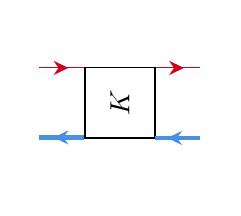
\begin{tikzpicture}[x=0.75pt,y=0.75pt,yscale=-1,xscale=1, baseline=(XXXX.south) ]
\path (0,77);\path (89.33333587646484,0);\draw    ($(current bounding box.center)+(0,0.3em)$) node [anchor=south] (XXXX) {};
%Straight Lines [id:da7115676979609427] 
\draw [color={rgb, 255:red, 208; green, 2; blue, 27 }  ,draw opacity=1 ]   (5.5,19.39) -- (27.61,19.39) ;
%Straight Lines [id:da8226174984587384] 
\draw [color={rgb, 255:red, 208; green, 2; blue, 27 }  ,draw opacity=1 ]   (61.36,19.39) -- (83.06,19.39) ;
%Straight Lines [id:da25326861646368304] 
\draw [color={rgb, 255:red, 208; green, 2; blue, 27 }  ,draw opacity=1 ]   (16.56,19.39) -- (16.61,19.39) ;
\draw [shift={(19.61,19.39)}, rotate = 180] [fill={rgb, 255:red, 208; green, 2; blue, 27 }  ,fill opacity=1 ][line width=0.08]  [draw opacity=0] (7.14,-3.43) -- (0,0) -- (7.14,3.43) -- (4.74,0) -- cycle    ;
%Straight Lines [id:da34362814096939687] 
\draw [color={rgb, 255:red, 208; green, 2; blue, 27 }  ,draw opacity=1 ]   (72.21,19.39) -- (72.27,19.39) ;
\draw [shift={(75.27,19.39)}, rotate = 180] [fill={rgb, 255:red, 208; green, 2; blue, 27 }  ,fill opacity=1 ][line width=0.08]  [draw opacity=0] (7.14,-3.43) -- (0,0) -- (7.14,3.43) -- (4.74,0) -- cycle    ;
%Shape: Square [id:dp2058159278792857] 
\draw   (27.61,19.39) -- (61.36,19.39) -- (61.36,53.14) -- (27.61,53.14) -- cycle ;
%Straight Lines [id:da7878855943317369] 
\draw [color={rgb, 255:red, 74; green, 144; blue, 226 }  ,draw opacity=1 ][line width=1.5]    (61.36,53.14) -- (83.06,53.14) ;
%Straight Lines [id:da23573675788589998] 
\draw [color={rgb, 255:red, 74; green, 144; blue, 226 }  ,draw opacity=1 ]   (72.21,53.14) -- (70.27,53.14) ;
\draw [shift={(67.27,53.14)}, rotate = 360] [fill={rgb, 255:red, 74; green, 144; blue, 226 }  ,fill opacity=1 ][line width=0.08]  [draw opacity=0] (7.14,-3.43) -- (0,0) -- (7.14,3.43) -- (4.74,0) -- cycle    ;
%Straight Lines [id:da18492619986102254] 
\draw [color={rgb, 255:red, 74; green, 144; blue, 226 }  ,draw opacity=1 ][line width=1.5]    (5.64,52.89) -- (27.33,52.89) ;
%Straight Lines [id:da9508478089699361] 
\draw [color={rgb, 255:red, 74; green, 144; blue, 226 }  ,draw opacity=1 ]   (13.48,52.89) ;
\draw [shift={(12.54,52.89)}, rotate = 360] [fill={rgb, 255:red, 74; green, 144; blue, 226 }  ,fill opacity=1 ][line width=0.08]  [draw opacity=0] (7.14,-3.43) -- (0,0) -- (7.14,3.43) -- (4.74,0) -- cycle    ;
% Text Node
\draw (44.49,36.26) node  [rotate=-270]  {$K$};
\end{tikzpicture}
    \end{equation}
    
    simplest single-electron theory: quantum Boltzmann equation (QBE) 
}

\end{frame}

\begin{frame}
    \frametitle{Overview}

    \onslide<1->{
        \textbf{What to investigate} 

        Stable oscillation modes of QBE ($\Leftrightarrow$ infinite response to external field
        $\Leftrightarrow$ bosonic mode): for $n_{\vb*{p} \sigma \sigma'}(\vb*{r})$,
        $\varepsilon_{\vb*{p} \sigma \sigma'} = \varepsilon[\var{n}]$,
        \begin{equation}
            \pdv{n_{\vb*{p} }}{t} 
            + \underbrace{\pdv{\varepsilon_{\vb*{p} }}{\vb*{p}} \cdot \pdv{n_{\vb*{p} }}{\vb*{r}}}_{\text{diffusion}}
            \underbrace{- \pdv{\varepsilon_{\vb*{p} }}{\vb*{r}} \cdot \pdv{n_{\vb*{p} }}{\vb*{p}}}_{\text{force}}
            + \underbrace{\ii \comm*{\varepsilon_{\vb*{p}}}{n_{\vb*{p}}}}_{\text{multi-band}}
            = \underbrace{I_{\text{Fermi golden rule}}}_{\text{collision}} .
        \end{equation}
    }
    
    \onslide<2->{
        \vspace{0.5cm}

        \textbf{What to expect}
    
        Three types of important bosonic modes:
        
        \begin{itemize}
            \item Zero sound in uncharged single-band Fermi liquid
            \item Plasmon in charged single-band Fermi liquid = zero sound + long range interaction 
            \item Exciton in charged multi-band Fermi liquid
        \end{itemize}
    }
    
\end{frame}

\section{Zero sound}

\begin{frame}
\frametitle{Equation governing zero sound}

\onslide<1->{
    \textbf{System} Single-band Fermi liquid with spin ignored 
}

\onslide<2->{
    \vspace{0.5cm}

    \textbf{Kinetics of uncharged Fermi liquid} \emph{Landau equation} = QBE + 
    \begin{equation}
        \varepsilon_{\vb*{p}}(\vb*{r}) = \varepsilon^0_{\vb*{p}}
        + \frac{1}{V} \sum_{\vb*{p}'} f_{\vb*{p} \vb*{p}'} \var{n}_{\vb*{p}}(\vb*{r}) 
    \end{equation}
    
    (assumption: $\vb*{q} \to 0$ in $c^\dagger_{\vb*{p} + \vb*{q}} c_{\vb*{p}}$, 
    i.e. $\var{n}_{\vb*{p}}(\vb*{r})$ being smooth in $\vb*{r}$)
}

\onslide<3->{
    \vspace{0.5cm}

    \textbf{EOM governing zero sound} Small disturbance, no collision, :
    
    \begin{equation}
        \pdv{\var{n}_{\vb*{p}}}{t} 
        + \pdv{\varepsilon^{\text{static}}_{\vb*{p}}}{\vb*{p}} 
        \cdot \pdv{\var{n}_{\vb*{p}}}{\vb*{r}}
        - \pdv{n^{\text{static}}_{\vb*{p}}}{\vb*{p}} \cdot 
        \underbrace{\frac{1}{V} \sum_{\vb*{p}'} f_{\vb*{p} \vb*{p}'} \pdv{\var{n_{\vb*{p}}}}{\vb*{r}}}_{\pdv*{\varepsilon_{\vb*{p}}}{\vb*{r}}} = 0
    \end{equation}
}

\end{frame}

\begin{frame}
\frametitle{Fermi surface vibration}

\textbf{Ansatz} Disturbance as small as possible \dots
\begin{equation}
    {n}_{\vb*{p}}(\vb*{r}, t) = \ee^{\ii (\vb*{q} \cdot \vb*{r} - \ii \omega t)} 
    \theta(\mu - \varepsilon_{\vb*{p}}^{\text{stable}} - h(\vu*{p}))
\end{equation}    

\begin{center}
    

\tikzset{every picture/.style={line width=0.75pt}} %set default line width to 0.75pt        

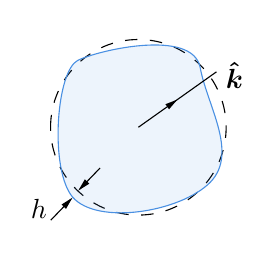
\begin{tikzpicture}[x=0.75pt,y=0.75pt,yscale=-0.5,xscale=0.5]
%uncomment if require: \path (0,300); %set diagram left start at 0, and has height of 300

%Shape: Circle [id:dp01917491317166009] 
\draw  [dash pattern={on 4.5pt off 4.5pt}] (121.52,175.11) .. controls (121.52,128.4) and (159.4,90.52) .. (206.11,90.52) .. controls (252.83,90.52) and (290.71,128.4) .. (290.71,175.11) .. controls (290.71,221.83) and (252.83,259.71) .. (206.11,259.71) .. controls (159.4,259.71) and (121.52,221.83) .. (121.52,175.11) -- cycle ;
%Shape: Polygon Curved [id:ds19124968571483536] 
\draw  [color={rgb, 255:red, 74; green, 144; blue, 226}, fill={rgb, 255:red, 74; green, 144; blue, 226}  ,fill opacity=0.1 ] (147.71,110.66) .. controls (167.71,100.66) and (258.71,79.66) .. (265.71,117.66) .. controls (272.71,155.66) and (304.71,202.66) .. (272.71,230.66) .. controls (240.71,258.66) and (160.71,269.66) .. (140.71,239.66) .. controls (120.71,209.66) and (127.71,120.66) .. (147.71,110.66) -- cycle ;
%Straight Lines [id:da9840179317331423] 
\draw    (206.11,175.11) -- (281.38,121.67) ;
\draw [shift={(243.75,148.39)}, rotate = 504.62] [fill={rgb, 255:red, 0; green, 0; blue, 0 }  ][line width=0.08]  [draw opacity=0] (12,-3) -- (0,0) -- (12,3) -- cycle    ;
%Straight Lines [id:da9902953526542171] 
\draw    (121.71,264.66) -- (141.19,244.42) ;
\draw [shift={(142.58,242.98)}, rotate = 493.92] [fill={rgb, 255:red, 0; green, 0; blue, 0 }  ][line width=0.08]  [draw opacity=0] (12,-3) -- (0,0) -- (12,3) -- cycle    ;
%Straight Lines [id:da6416680662048091] 
\draw    (169.25,214.31) -- (149.76,234.55) ;
\draw [shift={(148.37,235.99)}, rotate = 313.91999999999996] [fill={rgb, 255:red, 0; green, 0; blue, 0 }  ][line width=0.08]  [draw opacity=0] (12,-3) -- (0,0) -- (12,3) -- cycle    ;

% Text Node
\draw (100,242) node [anchor=north west][inner sep=0.75pt]    {$h$};
% Text Node
\draw (287.96,109.72) node [anchor=north west][inner sep=0.75pt]    {$\vu*{k}$};


\end{tikzpicture}

\end{center}

\textbf{Eigenvalue problem} \begin{equation}
    (\omega - \vb*{q} \cdot \vb*{v}) h(\vu*{k})
    = \vb*{q} \cdot \vb*{v} \int \frac{\dd{\Omega}'}{4\pi} F(\vartheta) h(\vu*{k}').
\end{equation}
where $\vb*{v}$ is single-electron velocity. $\Rightarrow$ zero sound has linear dispersion;
zero sound requires $F \neq 0$

\end{frame}

\begin{frame}
\frametitle{Modes}

\textbf{Shape of Fermi surface}

\begin{center}
    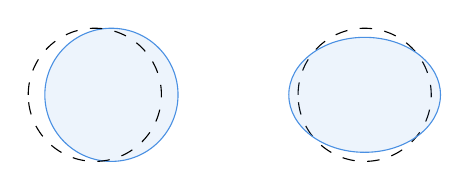
\begin{tikzpicture}[x=0.75pt,y=0.75pt,yscale=-1,xscale=1]
    %uncomment if require: \path (0,300); %set diagram left start at 0, and has height of 300
    %Shape: Circle [id:dp4755709967210189] 
    \draw  [color={rgb, 255:red, 74; green, 144; blue, 226 }  ,draw opacity=1 ][fill={rgb, 255:red, 74; green, 144; blue, 226 }  ,fill opacity=0.1 ] (100,166.52) .. controls (100,148.8) and (114.36,134.44) .. (132.08,134.44) .. controls (149.8,134.44) and (164.17,148.8) .. (164.17,166.52) .. controls (164.17,184.24) and (149.8,198.6) .. (132.08,198.6) .. controls (114.36,198.6) and (100,184.24) .. (100,166.52) -- cycle ;
    %Shape: Circle [id:dp35274170261087034] 
    \draw  [dash pattern={on 4.5pt off 4.5pt}] (92,166.52) .. controls (92,148.8) and (106.36,134.44) .. (124.08,134.44) .. controls (141.8,134.44) and (156.17,148.8) .. (156.17,166.52) .. controls (156.17,184.24) and (141.8,198.6) .. (124.08,198.6) .. controls (106.36,198.6) and (92,184.24) .. (92,166.52) -- cycle ;
    %Shape: Circle [id:dp12780434757124337] 
    \draw  [dash pattern={on 4.5pt off 4.5pt}] (222,166.52) .. controls (222,148.8) and (236.36,134.44) .. (254.08,134.44) .. controls (271.8,134.44) and (286.17,148.8) .. (286.17,166.52) .. controls (286.17,184.24) and (271.8,198.6) .. (254.08,198.6) .. controls (236.36,198.6) and (222,184.24) .. (222,166.52) -- cycle ;
    %Shape: Ellipse [id:dp307765088701216] 
    \draw  [color={rgb, 255:red, 74; green, 144; blue, 226 }  ,draw opacity=1 ][fill={rgb, 255:red, 74; green, 144; blue, 226 }  ,fill opacity=0.1 ] (217.54,166.52) .. controls (217.54,151.22) and (233.9,138.82) .. (254.08,138.82) .. controls (274.26,138.82) and (290.62,151.22) .. (290.62,166.52) .. controls (290.62,181.82) and (274.26,194.22) .. (254.08,194.22) .. controls (233.9,194.22) and (217.54,181.82) .. (217.54,166.52) -- cycle ;
\end{tikzpicture}    
\end{center}

\textbf{Distortion} More electrons in $\vu*{q}$; less electrons in $- \vu*{q}$

\begin{center}
    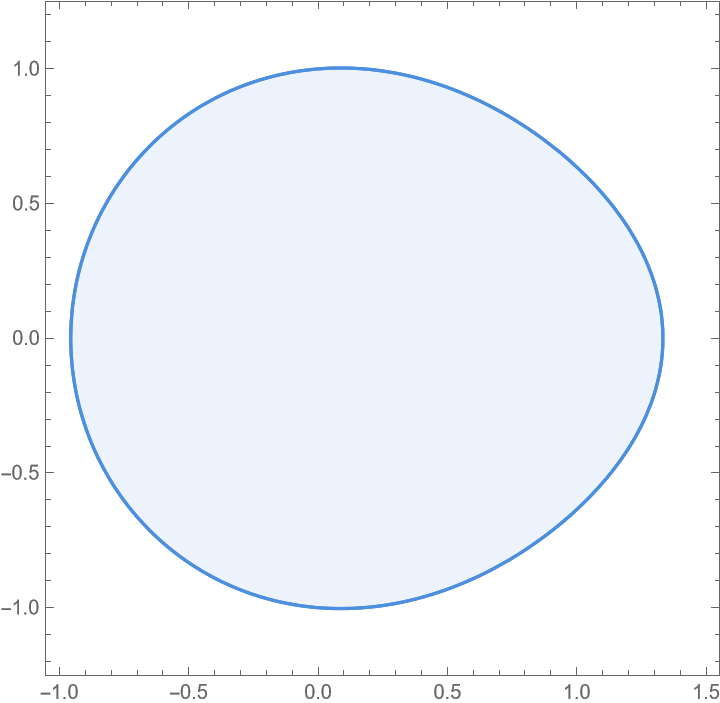
\includegraphics[width=0.2\textwidth]{spatial/zero-sound-l-0.png}
\end{center}

\textbf{Zero sound is not density wave} In zero sound $V_{\text{Fermi sea}} = \text{const}.$
$\Rightarrow$ zero sound is not ordinary sound

\end{frame}

\begin{frame}
\frametitle{Comparison with ordinary sound}

\textbf{Ordinary sound} Fermi liquid theory $\Rightarrow$ $\pdv*{\rho}{P}$ $\Rightarrow$
another sound mode (``first sound'', ordinary sound, density mode) from hydrodynamics

\vspace{0.5cm}

\textbf{Relation with zero sound} 
\begin{itemize}
    \item First sound appears when $\omega \tau \ll 1$:
    ordinary hydrodynamics $\Leftrightarrow$ local equilibrium $\Leftrightarrow$ $\tau \ll 1 / \omega$
    \item zero sound appears when $\omega \tau \gg 1$: 
    no collision integral $\Leftrightarrow$ $\tau \gg 1 / \omega$
\end{itemize}

The two are connected: a radical finite-$T$ correction

\begin{center}
    

% Gradient Info
  
\tikzset {_ia6lve64y/.code = {\pgfsetadditionalshadetransform{ \pgftransformshift{\pgfpoint{0 bp } { 0 bp }  }  \pgftransformrotate{-146 }  \pgftransformscale{2 }  }}}
\pgfdeclarehorizontalshading{_m7k45w8s4}{150bp}{rgb(0bp)=(1,1,1);
rgb(56.84058598109654bp)=(1,1,1);
rgb(59.8930413382394bp)=(0.61,0.61,0.61);
rgb(62.5bp)=(0.29,0.29,0.29);
rgb(100bp)=(0.29,0.29,0.29)}

% Gradient Info
  
\tikzset {_djogr69oa/.code = {\pgfsetadditionalshadetransform{ \pgftransformshift{\pgfpoint{0 bp } { 0 bp }  }  \pgftransformrotate{-129 }  \pgftransformscale{2 }  }}}
\pgfdeclarehorizontalshading{_p2j1wxwq4}{150bp}{rgb(0bp)=(0.29,0.29,0.29);
rgb(37.5bp)=(0.29,0.29,0.29);
rgb(43.7797600882394bp)=(1,1,1);
rgb(100bp)=(1,1,1)}
\tikzset{every picture/.style={line width=0.75pt}} %set default line width to 0.75pt        

\begin{tikzpicture}[x=0.75pt,y=0.75pt,yscale=-0.6,xscale=0.6]
%uncomment if require: \path (0,300); %set diagram left start at 0, and has height of 300

%Straight Lines [id:da6006990507896193] 
\draw    (257.92,94.17) -- (325.92,33.1) ;
%Straight Lines [id:da8463599501793553] 
\draw    (103,235) -- (344.17,235) ;
\draw [shift={(346.17,235)}, rotate = 180] [fill={rgb, 255:red, 0; green, 0; blue, 0 }  ][line width=0.08]  [draw opacity=0] (12,-3) -- (0,0) -- (12,3) -- cycle    ;
%Straight Lines [id:da2275445831732943] 
\draw    (103,235) -- (103,21.19) ;
\draw [shift={(103,19.19)}, rotate = 90] [fill={rgb, 255:red, 0; green, 0; blue, 0 }  ][line width=0.08]  [draw opacity=0] (12,-3) -- (0,0) -- (12,3) -- cycle    ;
%Straight Lines [id:da6099852885108679] 
\draw    (103,235) -- (184.26,201.02) ;
%Shape: Polygon Curved [id:ds3933722880021524] 
\draw  [draw opacity=0][shading=_m7k45w8s4,_ia6lve64y] (294.51,202.92) .. controls (242.83,207.29) and (203.28,197.08) .. (165.26,208.96) .. controls (197.68,188.2) and (225.06,176.75) .. (250.35,126.15) .. controls (261.8,137.72) and (295.13,166.87) .. (294.51,202.92) -- cycle ;
%Straight Lines [id:da7618060721275304] 
\draw  [dash pattern={on 0.84pt off 2.51pt}]  (103,235) -- (325.17,141.52) ;
%Shape: Polygon Curved [id:ds9419710356804576] 
\draw  [draw opacity=0][shading=_p2j1wxwq4,_djogr69oa] (171.32,89.99) .. controls (221.15,75.65) and (263.94,80.05) .. (296.92,58.92) .. controls (278.92,90.85) and (239.92,111.85) .. (229.57,156.7) .. controls (216.08,147.58) and (177.72,125.47) .. (171.32,89.99) -- cycle ;
%Straight Lines [id:da4615538031472426] 
\draw  [dash pattern={on 0.84pt off 2.51pt}]  (103,235) -- (326.17,32.85) ;
%Curve Lines [id:da7468246422953644] 
\draw  [dash pattern={on 4.5pt off 4.5pt}]  (184.26,201.02) .. controls (277.17,162.61) and (206.17,142.19) .. (291.92,63.64) ;
%Straight Lines [id:da9243960083758465] 
\draw  [dash pattern={on 0.84pt off 2.51pt}]  (104,127) -- (337.17,127) ;

% Text Node
\draw (328.17,35.85) node [anchor=north west][inner sep=0.75pt]   [align=left] {zero sound};
% Text Node
\draw (327.17,144.52) node [anchor=north west][inner sep=0.75pt]   [align=left] {first sound};
% Text Node
\draw (348.17,235) node [anchor=west] [inner sep=0.75pt]    {$q$};
% Text Node
\draw (101,19.19) node [anchor=east] [inner sep=0.75pt]    {$\omega $};
% Text Node
\draw (193,47) node [anchor=north west][inner sep=0.75pt]   [align=left] {collision};
% Text Node
\draw (233,197) node [anchor=north west][inner sep=0.75pt]   [align=left] {lack of collision};
% Text Node
\draw (101,127.09) node [anchor=east] [inner sep=0.75pt]    {$\sim \frac{1}{\tau }$};


\end{tikzpicture}

\end{center}    

\end{frame}

\section{Plasmon}

\begin{frame}
\frametitle{What happens with long-range interaction}

\textbf{The origin of $f_{\vb*{p} \vb*{p}'}$} 

\begin{equation}
    \protectf_{\boldsymbol{kk} '} = \lim_{\vb*{q} \to 0} \tikzset{every picture/.style={line width=0.75pt}} %set default line width to 0.75pt        
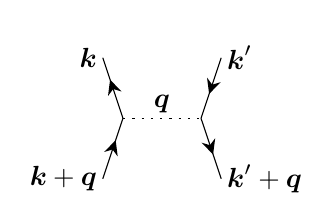
\begin{tikzpicture}[x=0.75pt,y=0.75pt,yscale=-0.8,xscale=0.8, baseline=(XXXX.south) ]
\path (0,100);\path (167,0);\draw    ($(current bounding box.center)+(0,0.3em)$) node [anchor=south] (XXXX) {};
%Straight Lines [id:da7098307100763392] 
\draw    (43.67,18.13) -- (55.83,54.56) ;
\draw [shift={(48.07,31.32)}, rotate = 71.54] [fill={rgb, 255:red, 0; green, 0; blue, 0 }  ][line width=0.08]  [draw opacity=0] (8.93,-4.29) -- (0,0) -- (8.93,4.29) -- (5.93,0) -- cycle    ;
%Straight Lines [id:da2424218861265588] 
\draw    (102.83,54.56) -- (115,91) ;
\draw [shift={(110.12,76.39)}, rotate = 251.54] [fill={rgb, 255:red, 0; green, 0; blue, 0 }  ][line width=0.08]  [draw opacity=0] (8.93,-4.29) -- (0,0) -- (8.93,4.29) -- (5.93,0) -- cycle    ;
%Straight Lines [id:da3743211626426439] 
\draw    (115,18.13) -- (102.83,54.56) ;
\draw [shift={(107.71,39.95)}, rotate = 288.46] [fill={rgb, 255:red, 0; green, 0; blue, 0 }  ][line width=0.08]  [draw opacity=0] (8.93,-4.29) -- (0,0) -- (8.93,4.29) -- (5.93,0) -- cycle    ;
%Straight Lines [id:da8496260309438608] 
\draw    (55.83,54.56) -- (43.67,91) ;
\draw [shift={(51.43,67.75)}, rotate = 108.46] [fill={rgb, 255:red, 0; green, 0; blue, 0 }  ][line width=0.08]  [draw opacity=0] (8.93,-4.29) -- (0,0) -- (8.93,4.29) -- (5.93,0) -- cycle    ;
%Straight Lines [id:da8568793968563864] 
\draw  [dash pattern={on 0.84pt off 2.51pt}]  (55.83,54.56) -- (102.83,54.56) ;
% Text Node
\draw (41.67,91) node [anchor=east] [inner sep=0.75pt]    {$\boldsymbol{k} +\boldsymbol{q}$};
% Text Node
\draw (41.67,18.13) node [anchor=east] [inner sep=0.75pt]    {$\boldsymbol{k}$};
% Text Node
\draw (117,18.13) node [anchor=west] [inner sep=0.75pt]    {$\boldsymbol{k} '$};
% Text Node
\draw (117,91) node [anchor=west] [inner sep=0.75pt]    {$\boldsymbol{k} '+\boldsymbol{q}$};
% Text Node
\draw (79.33,53.06) node [anchor=south] [inner sep=0.75pt]    {$\boldsymbol{q}$};
\end{tikzpicture}
+\tikzset{every picture/.style={line width=0.75pt}} %set default line width to 0.75pt        
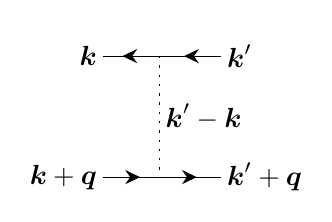
\begin{tikzpicture}[x=0.75pt,y=0.75pt,yscale=-0.8,xscale=0.8, baseline=(XXXX.south) ]
\path (0,100);\path (158.6666717529297,0);\draw    ($(current bounding box.center)+(0,0.3em)$) node [anchor=south] (XXXX) {};
%Straight Lines [id:da30879853278660363] 
\draw    (37.67,17.13) -- (71.93,17.13) ;
\draw [shift={(49.5,17.13)}, rotate = 0] [fill={rgb, 255:red, 0; green, 0; blue, 0 }  ][line width=0.08]  [draw opacity=0] (8.93,-4.29) -- (0,0) -- (8.93,4.29) -- (5.93,0) -- cycle    ;
%Straight Lines [id:da5722687884244773] 
\draw    (71.93,90) -- (109,90) ;
\draw [shift={(94.26,90)}, rotate = 180] [fill={rgb, 255:red, 0; green, 0; blue, 0 }  ][line width=0.08]  [draw opacity=0] (8.93,-4.29) -- (0,0) -- (8.93,4.29) -- (5.93,0) -- cycle    ;
%Straight Lines [id:da07387707354186368] 
\draw    (109,17.13) -- (71.93,17.13) ;
\draw [shift={(86.66,17.13)}, rotate = 360] [fill={rgb, 255:red, 0; green, 0; blue, 0 }  ][line width=0.08]  [draw opacity=0] (8.93,-4.29) -- (0,0) -- (8.93,4.29) -- (5.93,0) -- cycle    ;
%Straight Lines [id:da7965530508718655] 
\draw    (71.93,90) -- (37.67,90) ;
\draw [shift={(60.1,90)}, rotate = 180] [fill={rgb, 255:red, 0; green, 0; blue, 0 }  ][line width=0.08]  [draw opacity=0] (8.93,-4.29) -- (0,0) -- (8.93,4.29) -- (5.93,0) -- cycle    ;
%Straight Lines [id:da6483627859678205] 
\draw  [dash pattern={on 0.84pt off 2.51pt}]  (71.93,17.13) -- (71.93,90.1) ;
% Text Node
\draw (35.67,90) node [anchor=east] [inner sep=0.75pt]    {$\boldsymbol{k} +\boldsymbol{q}$};
% Text Node
\draw (35.67,17.13) node [anchor=east] [inner sep=0.75pt]    {$\boldsymbol{k}$};
% Text Node
\draw (111,17.13) node [anchor=west] [inner sep=0.75pt]    {$\boldsymbol{k} '$};
% Text Node
\draw (111,90) node [anchor=west] [inner sep=0.75pt]    {$\boldsymbol{k} '+\boldsymbol{q}$};
% Text Node
\draw (73.93,53.61) node [anchor=west] [inner sep=0.75pt]    {$\boldsymbol{k} '-\boldsymbol{k}$};
\end{tikzpicture}
\end{equation}

Coulomb interaction $\Rightarrow$ first term divergent in $\vb*{k}$ space
$\Rightarrow$ it should be considered in $\vb*{r}$ space 

\textbf{Landau-Silin eq.} 

\begin{equation}
    \pdv{n_{\vb*{p} }}{t} 
    + \pdv{\varepsilon_{\vb*{p} }}{\vb*{p}} \cdot \pdv{n_{\vb*{p} }}{\vb*{r}}
    - \pdv{(\varepsilon_{\vb*{p} } - e \varphi(\vb*{r}))}{\vb*{r}} \cdot \pdv{n_{\vb*{p} }}{\vb*{p}}
    = \underbrace{I_{\text{Fermi golden rule}}}_{\text{collision}} ,
\end{equation}
\begin{equation}
    \varepsilon_{\vb*{p}}(\vb*{r}) = \varepsilon^0_{\vb*{p}}
    + \frac{1}{V} \sum_{\vb*{p}'} f_{\vb*{p} \vb*{p}'} \var{n}_{\vb*{p}}(\vb*{r}) , \quad 
    \laplacian \varphi = e \cdot \frac{1}{V} \sum_{\vb*{p}} n_{\vb*{p}}(\vb*{r}).
\end{equation}

\end{frame}

\begin{frame}
\frametitle{Plasmon mode}

\textbf{Plasmon is gapped} When $\vb*{q} \to 0$ we get to the elementary case

\begin{center}
    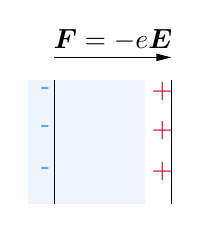
\begin{tikzpicture}[x=0.75pt,y=0.75pt,yscale=-0.6,xscale=0.6]
    %uncomment if require: \path (0,300); %set diagram left start at 0, and has height of 300
    
    %Straight Lines [id:da13477307007169825] 
    \draw    (100,123) -- (100,222.77) ;
    %Straight Lines [id:da43939624923609766] 
    \draw    (194,123) -- (194,222.77) ;
    %Shape: Rectangle [id:dp36771645669180764] 
    \draw  [draw opacity=0][fill={rgb, 255:red, 74; green, 144; blue, 226 }  ,fill opacity=0.1 ] (79,123) -- (173,123) -- (173,222.77) -- (79,222.77) -- cycle ;
    %Straight Lines [id:da5706192518127118] 
    \draw    (100,105) -- (192,105) ;
    \draw [shift={(194,105)}, rotate = 180] [fill={rgb, 255:red, 0; green, 0; blue, 0 }  ][line width=0.08]  [draw opacity=0] (12,-3) -- (0,0) -- (12,3) -- cycle    ;
    
    % Text Node
    \draw (87,123) node [anchor=north west][inner sep=0.75pt]  [color={rgb, 255:red, 74; green, 144; blue, 226 }  ,opacity=1 ] [align=left] {\mbox{-}};
    % Text Node
    \draw (87,154) node [anchor=north west][inner sep=0.75pt]  [color={rgb, 255:red, 74; green, 144; blue, 226 }  ,opacity=1 ] [align=left] {\mbox{-}};
    % Text Node
    \draw (87,187) node [anchor=north west][inner sep=0.75pt]  [color={rgb, 255:red, 74; green, 144; blue, 226 }  ,opacity=1 ] [align=left] {\mbox{-}};
    % Text Node
    \draw (176,123) node [anchor=north west][inner sep=0.75pt]  [color={rgb, 255:red, 208; green, 2; blue, 27 }  ,opacity=1 ] [align=left] {+};
    % Text Node
    \draw (176,154) node [anchor=north west][inner sep=0.75pt]  [color={rgb, 255:red, 208; green, 2; blue, 27 }  ,opacity=1 ] [align=left] {+};
    % Text Node
    \draw (176,187) node [anchor=north west][inner sep=0.75pt]  [color={rgb, 255:red, 208; green, 2; blue, 27 }  ,opacity=1 ] [align=left] {+};
    % Text Node
    \draw (147,102) node [anchor=south] [inner sep=0.75pt]    {$\boldsymbol{F} =-e\boldsymbol{E}$};
    
    
    \end{tikzpicture}
    
\end{center}
\begin{equation}
    m \ddot{\vb*{x}} = - m \omega^2 \vb*{x} = (- e) \vb*{E} = - e \cdot \frac{1}{\epsilon_0} e n \vb*{x} 
    \Rightarrow \omega = \sqrt{\frac{n e^2}{\epsilon_0 m}}.
\end{equation}

\vspace{0.25cm}

\textbf{Comparison with zero sound} When $\vb*{q} \to 0$, $\varphi(\vb*{r})$ $\Rightarrow$ oscillation:
long-range interaction $\Rightarrow$ finite gap

\vspace{0.25cm}

\textbf{Comparison with first sound} $V_{\text{Fermi sea}} = \text{const.}$ in plasmon as well:
plasmon is not a density mode

\end{frame}

\section{Exciton}

\section{Summary}

\begin{frame}
\frametitle{Summary}

\textbf{Fermi liquid, uncharged: zero sound} 
\begin{itemize}
    \item Linear, gapless 
    \item From $f_{\vb*{p} \vb*{p}'}$ 
\end{itemize}

\vspace{0.5cm}

\textbf{Fermi liquid, charged: plasmon} \begin{itemize}
    \item Divergent Hartree term $\Rightarrow$ self-energy correction in real space 
    \item When $\vb*{q} = 0$: $f_{\vb*{p} \vb*{p}'}$ not important; gapped
\end{itemize}

\vspace{0.5cm}

\textbf{Two bands: exciton} 

\end{frame}

\section{Further discussion}

\begin{frame}
\frametitle{Justifying quantum Boltzmann equation}

\textbf{Is QBE reliable?}

\emph{Yes!} When we intuitively expect it to work --

\begin{center}
    

\tikzset{every picture/.style={line width=0.75pt}} %set default line width to 0.75pt        

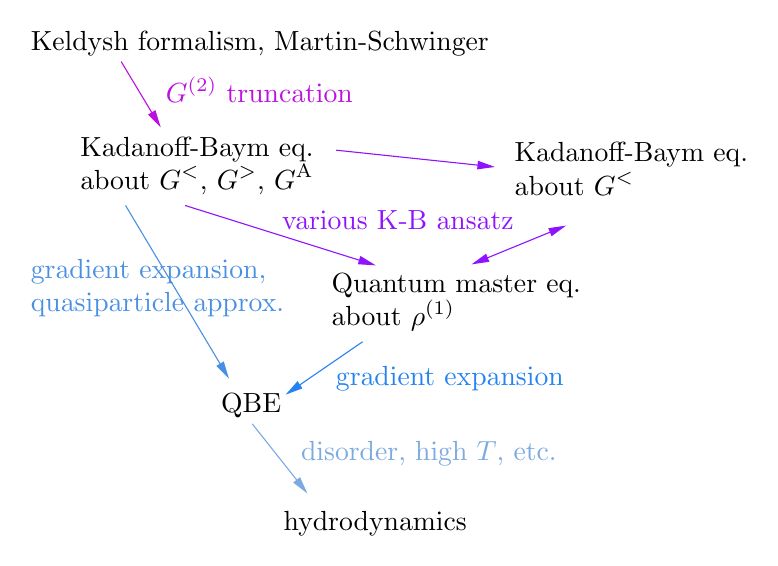
\begin{tikzpicture}[x=0.75pt,y=0.75pt,yscale=-0.7,xscale=0.7]
%uncomment if require: \path (0,409); %set diagram left start at 0, and has height of 409

%Straight Lines [id:da9993448313111608] 
\draw [color={rgb, 255:red, 189; green, 16; blue, 224 }  ,draw opacity=1 ]   (100,52) -- (126.14,95.47) ;
\draw [shift={(127.17,97.19)}, rotate = 238.99] [fill={rgb, 255:red, 189; green, 16; blue, 224 }  ,fill opacity=1 ][line width=0.08]  [draw opacity=0] (12,-3) -- (0,0) -- (12,3) -- cycle    ;
%Straight Lines [id:da505450204640074] 
\draw [color={rgb, 255:red, 144; green, 19; blue, 254 }  ,draw opacity=1 ]   (144,151) -- (273.26,191.59) ;
\draw [shift={(275.17,192.19)}, rotate = 197.43] [fill={rgb, 255:red, 144; green, 19; blue, 254 }  ,fill opacity=1 ][line width=0.08]  [draw opacity=0] (12,-3) -- (0,0) -- (12,3) -- cycle    ;
%Straight Lines [id:da7259646168352232] 
\draw [color={rgb, 255:red, 74; green, 144; blue, 226 }  ,draw opacity=1 ]   (103,151) -- (173.14,268.47) ;
\draw [shift={(174.17,270.19)}, rotate = 239.16] [fill={rgb, 255:red, 74; green, 144; blue, 226 }  ,fill opacity=1 ][line width=0.08]  [draw opacity=0] (12,-3) -- (0,0) -- (12,3) -- cycle    ;
%Straight Lines [id:da35768014069365206] 
\draw [color={rgb, 255:red, 36; green, 131; blue, 241 }  ,draw opacity=1 ]   (266.17,244.78) -- (214.82,280.06) ;
\draw [shift={(213.17,281.19)}, rotate = 325.51] [fill={rgb, 255:red, 36; green, 131; blue, 241 }  ,fill opacity=1 ][line width=0.08]  [draw opacity=0] (12,-3) -- (0,0) -- (12,3) -- cycle    ;
%Straight Lines [id:da15985835431985884] 
\draw [color={rgb, 255:red, 124; green, 170; blue, 224 }  ,draw opacity=1 ]   (190.17,301.25) -- (226.93,347.68) ;
\draw [shift={(228.17,349.25)}, rotate = 231.63] [fill={rgb, 255:red, 124; green, 170; blue, 224 }  ,fill opacity=1 ][line width=0.08]  [draw opacity=0] (12,-3) -- (0,0) -- (12,3) -- cycle    ;
%Straight Lines [id:da33183770683384806] 
\draw [color={rgb, 255:red, 144; green, 19; blue, 254 }  ,draw opacity=1 ]   (248,112.94) -- (355.18,124.25) ;
\draw [shift={(357.17,124.46)}, rotate = 186.02] [fill={rgb, 255:red, 144; green, 19; blue, 254 }  ,fill opacity=1 ][line width=0.08]  [draw opacity=0] (12,-3) -- (0,0) -- (12,3) -- cycle    ;
%Straight Lines [id:da43680180859475204] 
\draw [color={rgb, 255:red, 144; green, 19; blue, 254 }  ,draw opacity=1 ]   (404.32,165.61) -- (343.02,190.76) ;
\draw [shift={(341.17,191.52)}, rotate = 337.69] [fill={rgb, 255:red, 144; green, 19; blue, 254 }  ,fill opacity=1 ][line width=0.08]  [draw opacity=0] (12,-3) -- (0,0) -- (12,3) -- cycle    ;
\draw [shift={(406.17,164.85)}, rotate = 157.69] [fill={rgb, 255:red, 144; green, 19; blue, 254 }  ,fill opacity=1 ][line width=0.08]  [draw opacity=0] (12,-3) -- (0,0) -- (12,3) -- cycle    ;

% Text Node
\draw (36,29) node [anchor=north west][inner sep=0.75pt]   [align=left] {Keldysh formalism, Martin-Schwinger};
% Text Node
\draw (195.1,71.44) node  [color={rgb, 255:red, 189; green, 16; blue, 224 }  ,opacity=1 ] [align=left] {$\displaystyle G^{( 2)}$ truncation};
% Text Node
\draw (70,102) node [anchor=north west][inner sep=0.75pt]   [align=left] {Kadanoff-Baym eq.\\about $\displaystyle G^{< }$, $\displaystyle G^{ >}$, $\displaystyle G^{\text{A}}$};
% Text Node
\draw (209,153) node [anchor=north west][inner sep=0.75pt]  [color={rgb, 255:red, 144; green, 19; blue, 254 }  ,opacity=1 ] [align=left] {various K-B ansatz};
% Text Node
\draw (243,196) node [anchor=north west][inner sep=0.75pt]   [align=left] {Quantum master eq.\\about $\displaystyle \rho ^{( 1)}$};
% Text Node
\draw (36,186) node [anchor=north west][inner sep=0.75pt]  [color={rgb, 255:red, 74; green, 144; blue, 226 }  ,opacity=1 ] [align=left] {gradient expansion,\\quasiparticle approx.};
% Text Node
\draw (167,279) node [anchor=north west][inner sep=0.75pt]   [align=left] {QBE};
% Text Node
\draw (246,260) node [anchor=north west][inner sep=0.75pt]  [color={rgb, 255:red, 36; green, 131; blue, 241 }  ,opacity=1 ] [align=left] {gradient expansion};
% Text Node
\draw (222,311.45) node [anchor=north west][inner sep=0.75pt]  [color={rgb, 255:red, 124; green, 170; blue, 224 }  ,opacity=1 ] [align=left] {disorder, high $\displaystyle T$, etc.};
% Text Node
\draw (210,359.45) node [anchor=north west][inner sep=0.75pt]   [align=left] {hydrodynamics};
% Text Node
\draw (369,106) node [anchor=north west][inner sep=0.75pt]   [align=left] {Kadanoff-Baym eq.\\about $\displaystyle G^{< }$};


\end{tikzpicture}

\end{center}

\end{frame}

\begin{frame}
\frametitle{Discussion}



\end{frame}

\end{document}